\documentclass[11pt]{amsart}
\usepackage{geometry}                % See geometry.pdf to learn the layout options. There are lots.
\geometry{letterpaper}                   % ... or a4paper or a5paper or ... 
%\geometry{landscape}                % Activate for for rotated page geometry
%\usepackage[parfill]{parskip}    % Activate to begin paragraphs with an empty line rather than an indent
\usepackage{graphicx}
\usepackage{amssymb}
\usepackage{epstopdf}
\usepackage{subfigure}

\usepackage[latin1]{inputenc}
\usepackage{tikz}
\usetikzlibrary{scopes}


\DeclareGraphicsRule{.tif}{png}{.png}{`convert #1 `dirname #1`/`basename #1 .tif`.png}

\title{Oscilator: Simulaci\'{o}n de un movimiento libre amortiguado }
\author{Carlos L\'{o}pez Camey y Mart\'{i}n Guzm\'{a}n}
%\date{}                                           % Activate to display a given date or no date


\begin{document}
\maketitle


\begin{abstract}

        Dise\~{n}amos y constru\'{i}mos un simulador de un sistema masa-resorte en un movimiento libre amortiguado.
\end{abstract}

\section{Modelaje}

Consideremos un sistema-masa resorte, en donde un resorte flexible se suspende verticalmente de un soporte r\'{i}gido y luego se une una masa $m$ a su extremo libre. Existe tambi\'{e}n una fuerza amortiguada $F_{amortiguadora}$ considerada proporcional a la velocidad instant\'{a}nea del sistema $v$, digamos $F_{amortiguadora} = bv$. \\

\begin{figure}[htp]
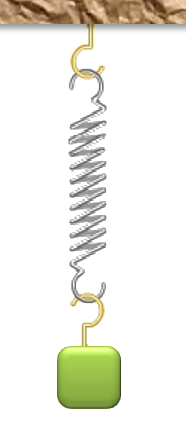
\includegraphics[scale=0.35]{img/screenshot.png}
\end{figure}

Sabemos que por la Ley de Hooke, el resorte ejerce una fuerza restauradora $F_{resorte} = ks$  opuesta a la direcci\'{o}n de alargamiento y proporcional a la cantidad de elongaci\'{o}n $s$ en donde $k$ es una constante de proporcionalidad llamada \textbf{constante de resorte}. 

En un diagrama de cuerpo libre, tenemos 

\begin{center}
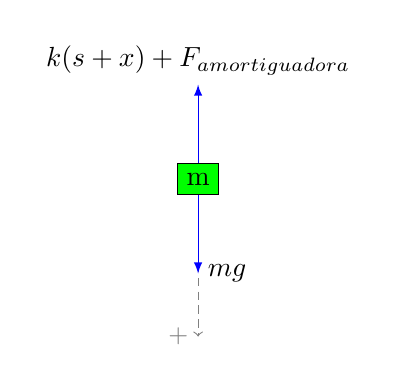
\begin{tikzpicture}[
    force/.style={>=latex,draw=blue,fill=blue},
    axis/.style={densely dashed,gray,font=\small},
    M/.style={rectangle,draw,fill=lightgray,minimum size=0.5cm,thin},
    m/.style={rectangle,draw=black,fill=green,minimum size=0.3cm,thin},
    plane/.style={draw=black,fill=blue!10},
    string/.style={draw=red, thick},
    pulley/.style={thick},
]

\matrix[column sep=1cm] {
    
    %%%
    % Free body diagram of m
    \node[m] (m) {m};
    \draw[axis,->] (m) -- ++(0,-2) node[left] {$+$};
    {[force,->]
        \draw (m.north) -- ++(0,1) node[above] {$k(s+x) + F_{amortiguadora}$};
        \draw (m.south) -- ++(0,-1) node[right] {$mg$};
    }

\\
};
\end{tikzpicture}
\end{center}

Deducimos por la segunda ley de Newton que
\[ma = mg - k(s+x) - F_{amortiguadora}  = mg - ks - kx - F_{amortiguadora}\]

Notemos que los t\'{e}rminos $mg$ y $ks$ son iguales en $t=0$, por lo que
\[ma = -kx - F_{amortiguadora}\]
\[ma + bv  + kx = 0\]

Escrito de otra forma, 
\begin{equation}
my''  + by' + kx = 0
\label{eq1}
\end{equation}

Con condiciones iniciales $y(0) = s = x_o$ y $y'(0) = v_o$

\vspace{1cm}
\section{Soluci\'{o}n}

Re-escribiendo (\ref{eq1}) tenemos:
\begin{equation}
y'' + 2\lambda y' + \omega^2 y =0 
\label{eqn:zill}
\end{equation}

en donde escogemos $2\lambda = \frac{b}{m}$ y $\omega^2 = \frac{k}{m}$ por conveniencia algebra\'{i}ca.  \\

Tenemos una ecuaci\'{o}n lineal homog\'{e}nea con coeficientes constantes, cuyo polinomio caracter\'{i}stico es 

\[ m^2 + 2\lambda m + \omega^2 = 0\]

con ra\'{i}ces en 
\[ m_1 = -\lambda + \sqrt{\lambda^2-\omega^2}\]
\[ m_2 = -\lambda - \sqrt{\lambda^2-\omega^2}\]

Observemos que $\lambda^2 - \omega^2  = \frac{b^2}{4m^2} - \frac{k}{m} = b^2 - 4mk$.

Notemos entonces que existen tres diferentes casos para las ra\'{i}ces i.e. soluciones

\vspace{1cm}


\subsection{Caso 1:} 
Si $\lambda^2 - \omega^2>0$ entonces, tenemos dos soluciones reales y decimos que el sistema est\'{a} \textbf{sobreamortiguado}, por que el coeficiente de amortiguamiento $b$ es grande comparado con la constante de resorte $k$. La soluci\'{o}n correspondiente a \ref{eqn:zill} y por consiguiente a la expresi\'{o}n que modela el movimiento en funci\'{o}n del tiempo es,

\[ y(t) = c_1e^{m_1t}+c_2e^{m_2t}\]

En donde sabemos que $y(0) = x_o$, por lo tanto

\[ y(0) = x_o = c_1 + c_2 \implies c_1 = x_o - c_2\]

Derivando (\ref{eqn:zill}), tenemos

\[ y'(t) = c_1m_1e^{m_1t} + c_2m_2e^{m_2t} \]


Y dadas las condiciones iniciales, podemos evaluar en $t=0$, que

\[ y'(0) = v_o = c_1m_1 + c_2m_2\]

Substituyendo $c_1 = x_o - c_2$

\[ v_o = (x_o - c_2)m_1 + c_2m_2 \]

\[ \implies c_2 = \frac{v_o - x_om_1}{m_2-m_1}\]

Notemos que $c_1$ y $c_2$ est\'{a}n en t\'{e}rminos de las condiciones del problema. 

\vspace{1cm}

\subsection{Caso 2:}
Si $\lambda^2 - \omega^2=0$ entonces, decimos que el sistema est\'{a} cr\'{i}ticamente amortiguado y tenemos una soluci\'{o}n real, por lo que la soluci\'{o}n correspondiente ser\'{i}a 

\[ y(t) = c_1e^{m_1t} + c_2te^{m_1t}\]

e inmediatamente vemos que

\[ y(0)  = c_1 =  x_o\]

De nuevo, derivando la soluci\'{o}n $y(t)$, tenemos la expresi\'{o}n que modela a la velocidad de este respecto al tiempo

\[ y'(t) = c_1m_1e^{m_1t} + c_2[m_1te^{m_1t} + e^{m_1t}]\]

que dadas las condiciones iniciales, tenemos

\[ y'(0) = x_om_1 + c2 = v_o \]

\[ \implies c_2 = v_o - x_om_1\]


\vspace{1cm}
\subsection{Caso 3:}
Si $\lambda^2 - \omega^2 < 0$, decimos que el sistema est\'{a} subamortiguado, puesto que el coeficiente de amortiguamiento es peque\~{n}o comparado con la constante del resorte. Las ra\'{i}ces ahora son complejas:

\[ m_1 = -\lambda + \sqrt{\lambda^2-\omega^2}  i\]
\[ m_2 = -\lambda - \sqrt{\lambda^2-\omega^2} i \]

As\'{i} que la ecuaci\'{o}n general de (\ref{eqn:zill}) en este caso es,

\[ y(t) = e^{-\lambda t}(c_1\cos{\beta t} + c_2\sin{\beta t} )\]

en donde $\beta = \sqrt{\lambda^2 - \omega^2}$ 

Entonces,

\[ y'(t) = -\lambda e^t (c_1\cos{\beta t} + c_2\sin{\beta t}) + e^{-\lambda t} \beta(-c_1 \sin{\beta t} + c_2 \cos{\beta t})\]

Por lo tanto,

\[ y(0) = c_1 = x_o\]

y

\[ y'(0) = -\lambda c_1 + c_2\beta \]

\[ \implies c_2  = \frac{v_o+\lambda x_o}{\beta}\]

Tenemos entonces, para cualquiera de los tres casos, una funci\'{o}n soluci\'{o}n $y(t)$ en funci\'{o}n de las condiciones iniciales y de las caracter\'{i}sticas del resorte, fuerza amortiguadora y la masa relacionada. \\

\vspace{1cm}
\section {Simulaci\'{o}n}

Para la simulaci\'{o}n, tuvimos que hacerla por medio de 4 im\'{a}genes separadas: El gancho de arriba, el resorte, el gancho de abajo y la masa.
\vspace*{-0.75in}
\begin{figure}[htp]
  \begin{center}
    \subfigure{\label{fig:gancho-abajo}\includegraphics[scale=0.45]{img/gancho_abajo_1.png}}
    \subfigure{\label{fig:gancho-arriba-b}\includegraphics[scale=0.45]{img/gancho_arriba_1.png}} 
    \subfigure{\label{fig:masa}
\includegraphics[scale=1.2]{img/masa2.png}}
     \subfigure{\label{fig:resorte}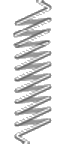
\includegraphics[scale=0.3]{img/resorte_1.png}}
  \end{center}
  \caption{Im\'{a}genes utilizadas}
\end{figure}

Cada una de estas concatenada a donde finalizaba la anterior, compon\'{i}an el sistema.

\vspace*{-0.025in}
\begin{figure}[htp]
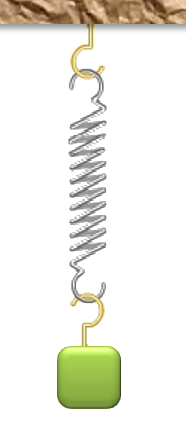
\includegraphics[scale=0.35]{img/screenshot.png}
\caption{Como luce el sistema "armado"}
\end{figure}

\subsection*{Algoritmo:} Se ten\'{i}a una variable que controlaba el tama\~{n}o vertical i.e. altura del resorte, dependiendo de la funci\'{o}n soluci\'{o}n $y(t)$. \\

Se ten\'{i}a un \textit{Timer} que corr\'{i}a cada 50 milisegundos y representaba a la variable independiente, $t$. Finalmente, lo que se hac\'{i}a era asignarle una escala al resultado de $y(t)$ para mejor visualizaci\'{o}n en pantalla. \\

El secreto estubo en irle cambiando el tama\~{n}o del resorte y siempre manteniendo la masa y el gancho al final de \'{e}ste

\section{Ejemplos}

\subsection{Sistema sobre-amortiguado}

Supongamos $m=1$, $b=3$, $k=1$ con condiciones iniciales $y(0) = 3$ y $y'(0) = 0$.\\

Tenemos entonces, el caso sobre-amortiguado ya que vemos que $b^2 > 4mk$, y por lo tanto las ra\'{i}ces del polinomio caracter\'{i}stico de la E.D. diferencial $y''(t) + 3y'(t) + y = 0$ que modela este caso, son dos soluciones reales distintas.\\

Entonces, la funci\'{o}n soluci\'{o}n del problema est\'{a} dada por
\[ y(t) = 3.512e^{\frac{-3+\sqrt{5}}{2}t} - 0.512e^{\frac{-3-\sqrt{5}}{2}t}\]

Y simulada, se ve de la siguiente manera
\begin{center}
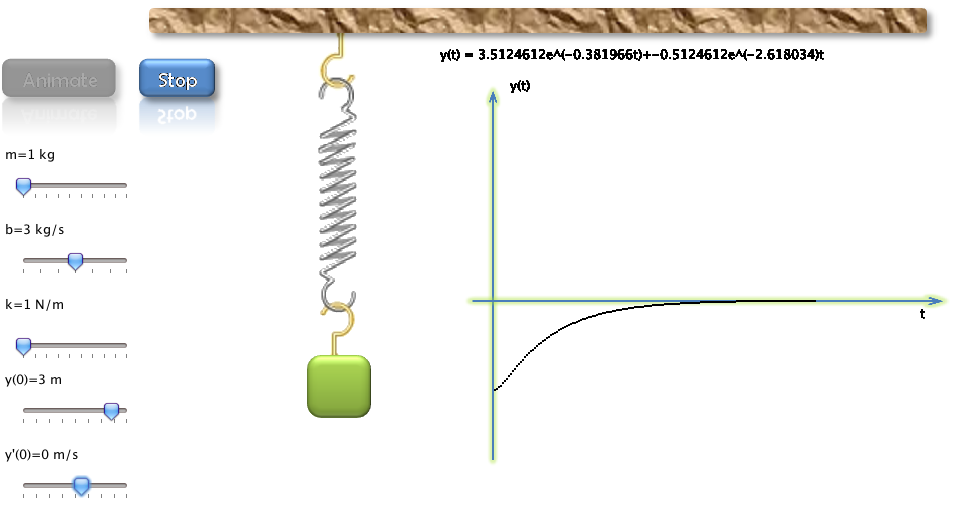
\includegraphics[scale=0.45]{img/ejemplo1.png}
\end{center}

\subsection{Sistema cr\'{i}ticamente-amortiguado}

Supongamos $m=4$, $b=4$, $k=1$ con condiciones iniciales $y(0) = 3$ y $y'(0) = -4$.\\

Tenemos entonces, el caso cr\'{i}ticamente-amortiguado ya que vemos que $b^2 = 4mk$, y por lo tanto las ra\'{i}ces del polinomio caracter\'{i}stico de la E.D. diferencial $4y''(t) + 4y'(t) + y = 0$ que modela este otro caso, son iguales\\

Entonces, la funci\'{o}n soluci\'{o}n del problema est\'{a} dada por
\[ y(t) = 3e^{-\frac{t}{2}} - \frac{5}{2}te^{-\frac{t}{2}} = e^{-\frac{t}{2}}(3-\frac{5}{2}t) \]

\begin{center}
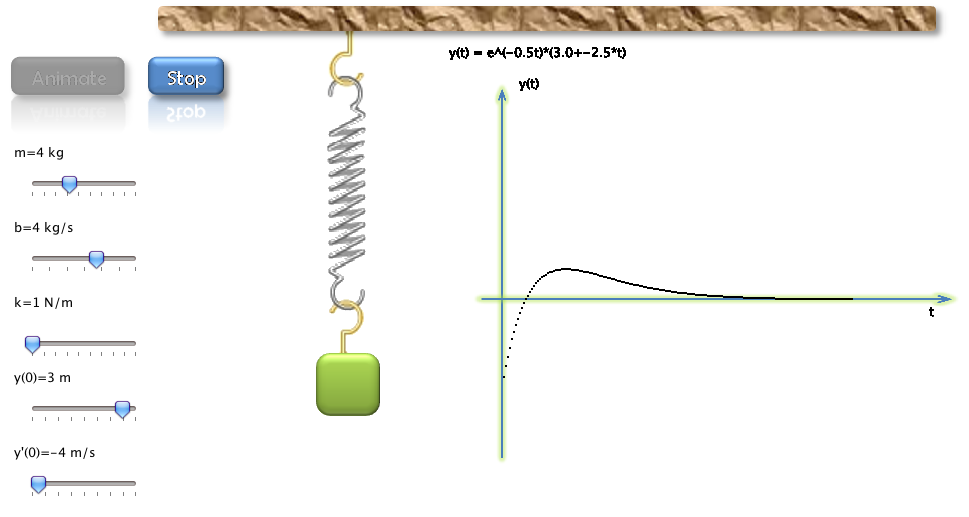
\includegraphics[scale=0.45]{img/ejemplo2.png}
\end{center}

\subsection{Sistema sub-amortiguado}

Supongamos $m=2$, $b=1$, $k=3$ con condiciones iniciales $y(0) = -4$ y $y'(0) = -1$.\\

Tenemos entonces, el caso sub-amortiguado ya que vemos que $b^2 < 4mk$, y por lo tanto las ra\'{i}ces del polinomio caracter\'{i}stico de la E.D. diferencial $2y''(t) + y'(t) + 3y = 0$ que modela este otro caso, son imaginarias.\\

Entonces, la funci\'{o}n soluci\'{o}n del problema est\'{a} dada por
\[ y(t) =  e^{-\frac{1}{4}t}(-4\cos{\frac{\sqrt{23}}{4}t} - \frac{8\sqrt{23}}{23}\sin{\frac{\sqrt{23}}{4}t})\]

\begin{center}
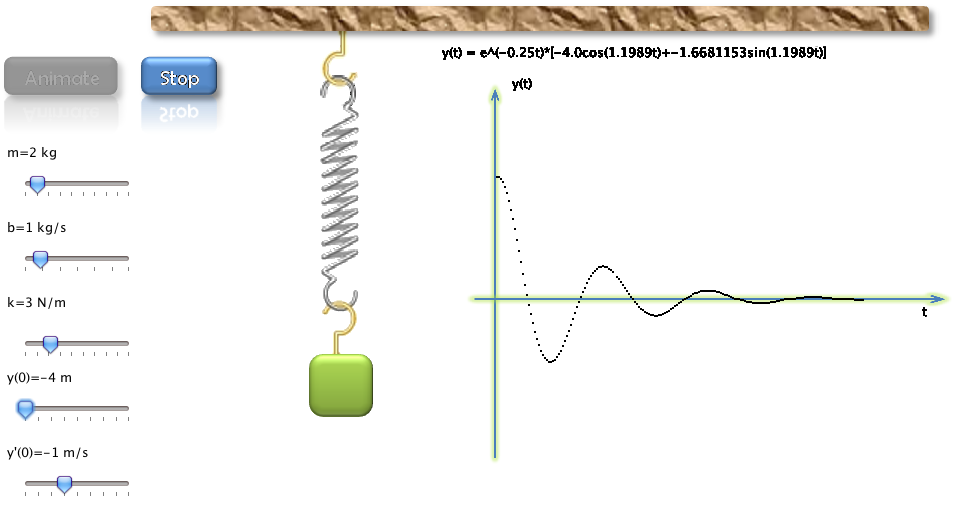
\includegraphics[scale=0.45]{img/ejemplo3.png}
\end{center}

\end{document}  


